% Quiver visualization of the 1-form d(z^2) = 2z dz on the complex plane:
% at each grid point, short arrows in the four axis directions are
% labeled with the value of the form on that tangent vector.
% Source: book/tex/riemann-surface/forms.tex (generated; edit the
% generator comment in the repo history rather than by hand).
\documentclass[border=2mm]{standalone}
\usepackage{tikz}
\usepackage{amsmath}
\begin{document}
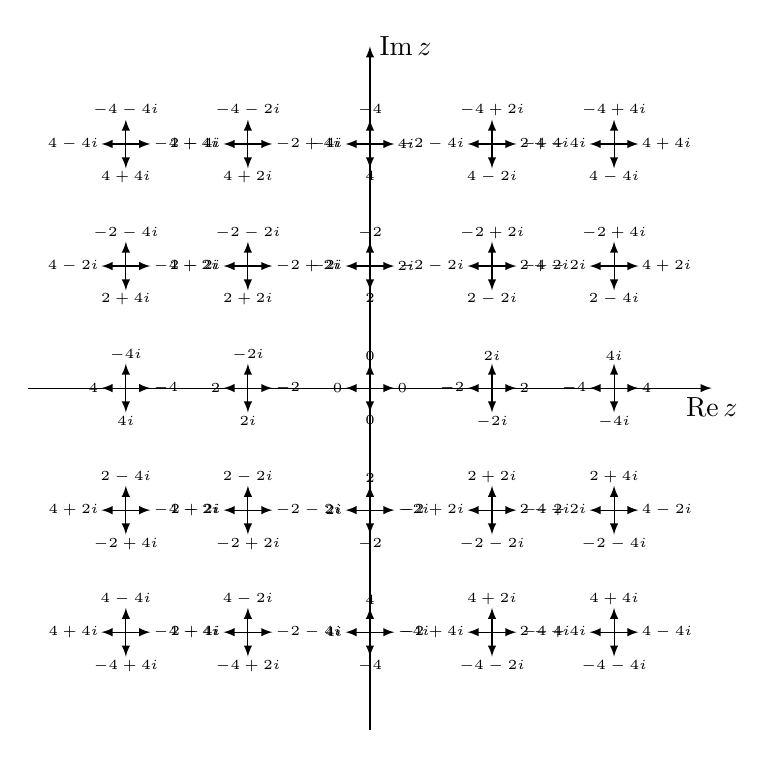
\begin{tikzpicture}[scale=1.55,>=latex]
  \draw[->] (-2.8,0) -- (2.8,0) node[below] {$\operatorname{Re} z$};
  \draw[->] (0,-2.8) -- (0,2.8) node[right] {$\operatorname{Im} z$};
  \draw[->] (-2,-2) -- (-1.8,-2) node[anchor=west, inner sep=1pt] {\tiny $-4-4i$};
  \draw[->] (-2,-2) -- (-2,-1.8) node[anchor=south, inner sep=1pt] {\tiny $4-4i$};
  \draw[->] (-2,-2) -- (-2.2,-2) node[anchor=east, inner sep=1pt] {\tiny $4+4i$};
  \draw[->] (-2,-2) -- (-2,-2.2) node[anchor=north, inner sep=1pt] {\tiny $-4+4i$};
  \draw[->] (-2,-1) -- (-1.8,-1) node[anchor=west, inner sep=1pt] {\tiny $-4-2i$};
  \draw[->] (-2,-1) -- (-2,-0.8) node[anchor=south, inner sep=1pt] {\tiny $2-4i$};
  \draw[->] (-2,-1) -- (-2.2,-1) node[anchor=east, inner sep=1pt] {\tiny $4+2i$};
  \draw[->] (-2,-1) -- (-2,-1.2) node[anchor=north, inner sep=1pt] {\tiny $-2+4i$};
  \draw[->] (-2,0) -- (-1.8,0) node[anchor=west, inner sep=1pt] {\tiny $-4$};
  \draw[->] (-2,0) -- (-2,0.2) node[anchor=south, inner sep=1pt] {\tiny $-4i$};
  \draw[->] (-2,0) -- (-2.2,0) node[anchor=east, inner sep=1pt] {\tiny $4$};
  \draw[->] (-2,0) -- (-2,-0.2) node[anchor=north, inner sep=1pt] {\tiny $4i$};
  \draw[->] (-2,1) -- (-1.8,1) node[anchor=west, inner sep=1pt] {\tiny $-4+2i$};
  \draw[->] (-2,1) -- (-2,1.2) node[anchor=south, inner sep=1pt] {\tiny $-2-4i$};
  \draw[->] (-2,1) -- (-2.2,1) node[anchor=east, inner sep=1pt] {\tiny $4-2i$};
  \draw[->] (-2,1) -- (-2,0.8) node[anchor=north, inner sep=1pt] {\tiny $2+4i$};
  \draw[->] (-2,2) -- (-1.8,2) node[anchor=west, inner sep=1pt] {\tiny $-4+4i$};
  \draw[->] (-2,2) -- (-2,2.2) node[anchor=south, inner sep=1pt] {\tiny $-4-4i$};
  \draw[->] (-2,2) -- (-2.2,2) node[anchor=east, inner sep=1pt] {\tiny $4-4i$};
  \draw[->] (-2,2) -- (-2,1.8) node[anchor=north, inner sep=1pt] {\tiny $4+4i$};
  \draw[->] (-1,-2) -- (-0.8,-2) node[anchor=west, inner sep=1pt] {\tiny $-2-4i$};
  \draw[->] (-1,-2) -- (-1,-1.8) node[anchor=south, inner sep=1pt] {\tiny $4-2i$};
  \draw[->] (-1,-2) -- (-1.2,-2) node[anchor=east, inner sep=1pt] {\tiny $2+4i$};
  \draw[->] (-1,-2) -- (-1,-2.2) node[anchor=north, inner sep=1pt] {\tiny $-4+2i$};
  \draw[->] (-1,-1) -- (-0.8,-1) node[anchor=west, inner sep=1pt] {\tiny $-2-2i$};
  \draw[->] (-1,-1) -- (-1,-0.8) node[anchor=south, inner sep=1pt] {\tiny $2-2i$};
  \draw[->] (-1,-1) -- (-1.2,-1) node[anchor=east, inner sep=1pt] {\tiny $2+2i$};
  \draw[->] (-1,-1) -- (-1,-1.2) node[anchor=north, inner sep=1pt] {\tiny $-2+2i$};
  \draw[->] (-1,0) -- (-0.8,0) node[anchor=west, inner sep=1pt] {\tiny $-2$};
  \draw[->] (-1,0) -- (-1,0.2) node[anchor=south, inner sep=1pt] {\tiny $-2i$};
  \draw[->] (-1,0) -- (-1.2,0) node[anchor=east, inner sep=1pt] {\tiny $2$};
  \draw[->] (-1,0) -- (-1,-0.2) node[anchor=north, inner sep=1pt] {\tiny $2i$};
  \draw[->] (-1,1) -- (-0.8,1) node[anchor=west, inner sep=1pt] {\tiny $-2+2i$};
  \draw[->] (-1,1) -- (-1,1.2) node[anchor=south, inner sep=1pt] {\tiny $-2-2i$};
  \draw[->] (-1,1) -- (-1.2,1) node[anchor=east, inner sep=1pt] {\tiny $2-2i$};
  \draw[->] (-1,1) -- (-1,0.8) node[anchor=north, inner sep=1pt] {\tiny $2+2i$};
  \draw[->] (-1,2) -- (-0.8,2) node[anchor=west, inner sep=1pt] {\tiny $-2+4i$};
  \draw[->] (-1,2) -- (-1,2.2) node[anchor=south, inner sep=1pt] {\tiny $-4-2i$};
  \draw[->] (-1,2) -- (-1.2,2) node[anchor=east, inner sep=1pt] {\tiny $2-4i$};
  \draw[->] (-1,2) -- (-1,1.8) node[anchor=north, inner sep=1pt] {\tiny $4+2i$};
  \draw[->] (0,-2) -- (0.2,-2) node[anchor=west, inner sep=1pt] {\tiny $-4i$};
  \draw[->] (0,-2) -- (0,-1.8) node[anchor=south, inner sep=1pt] {\tiny $4$};
  \draw[->] (0,-2) -- (-0.2,-2) node[anchor=east, inner sep=1pt] {\tiny $4i$};
  \draw[->] (0,-2) -- (0,-2.2) node[anchor=north, inner sep=1pt] {\tiny $-4$};
  \draw[->] (0,-1) -- (0.2,-1) node[anchor=west, inner sep=1pt] {\tiny $-2i$};
  \draw[->] (0,-1) -- (0,-0.8) node[anchor=south, inner sep=1pt] {\tiny $2$};
  \draw[->] (0,-1) -- (-0.2,-1) node[anchor=east, inner sep=1pt] {\tiny $2i$};
  \draw[->] (0,-1) -- (0,-1.2) node[anchor=north, inner sep=1pt] {\tiny $-2$};
  \draw[->] (0,0) -- (0.2,0) node[anchor=west, inner sep=1pt] {\tiny $0$};
  \draw[->] (0,0) -- (0,0.2) node[anchor=south, inner sep=1pt] {\tiny $0$};
  \draw[->] (0,0) -- (-0.2,0) node[anchor=east, inner sep=1pt] {\tiny $0$};
  \draw[->] (0,0) -- (0,-0.2) node[anchor=north, inner sep=1pt] {\tiny $0$};
  \draw[->] (0,1) -- (0.2,1) node[anchor=west, inner sep=1pt] {\tiny $2i$};
  \draw[->] (0,1) -- (0,1.2) node[anchor=south, inner sep=1pt] {\tiny $-2$};
  \draw[->] (0,1) -- (-0.2,1) node[anchor=east, inner sep=1pt] {\tiny $-2i$};
  \draw[->] (0,1) -- (0,0.8) node[anchor=north, inner sep=1pt] {\tiny $2$};
  \draw[->] (0,2) -- (0.2,2) node[anchor=west, inner sep=1pt] {\tiny $4i$};
  \draw[->] (0,2) -- (0,2.2) node[anchor=south, inner sep=1pt] {\tiny $-4$};
  \draw[->] (0,2) -- (-0.2,2) node[anchor=east, inner sep=1pt] {\tiny $-4i$};
  \draw[->] (0,2) -- (0,1.8) node[anchor=north, inner sep=1pt] {\tiny $4$};
  \draw[->] (1,-2) -- (1.2,-2) node[anchor=west, inner sep=1pt] {\tiny $2-4i$};
  \draw[->] (1,-2) -- (1,-1.8) node[anchor=south, inner sep=1pt] {\tiny $4+2i$};
  \draw[->] (1,-2) -- (0.8,-2) node[anchor=east, inner sep=1pt] {\tiny $-2+4i$};
  \draw[->] (1,-2) -- (1,-2.2) node[anchor=north, inner sep=1pt] {\tiny $-4-2i$};
  \draw[->] (1,-1) -- (1.2,-1) node[anchor=west, inner sep=1pt] {\tiny $2-2i$};
  \draw[->] (1,-1) -- (1,-0.8) node[anchor=south, inner sep=1pt] {\tiny $2+2i$};
  \draw[->] (1,-1) -- (0.8,-1) node[anchor=east, inner sep=1pt] {\tiny $-2+2i$};
  \draw[->] (1,-1) -- (1,-1.2) node[anchor=north, inner sep=1pt] {\tiny $-2-2i$};
  \draw[->] (1,0) -- (1.2,0) node[anchor=west, inner sep=1pt] {\tiny $2$};
  \draw[->] (1,0) -- (1,0.2) node[anchor=south, inner sep=1pt] {\tiny $2i$};
  \draw[->] (1,0) -- (0.8,0) node[anchor=east, inner sep=1pt] {\tiny $-2$};
  \draw[->] (1,0) -- (1,-0.2) node[anchor=north, inner sep=1pt] {\tiny $-2i$};
  \draw[->] (1,1) -- (1.2,1) node[anchor=west, inner sep=1pt] {\tiny $2+2i$};
  \draw[->] (1,1) -- (1,1.2) node[anchor=south, inner sep=1pt] {\tiny $-2+2i$};
  \draw[->] (1,1) -- (0.8,1) node[anchor=east, inner sep=1pt] {\tiny $-2-2i$};
  \draw[->] (1,1) -- (1,0.8) node[anchor=north, inner sep=1pt] {\tiny $2-2i$};
  \draw[->] (1,2) -- (1.2,2) node[anchor=west, inner sep=1pt] {\tiny $2+4i$};
  \draw[->] (1,2) -- (1,2.2) node[anchor=south, inner sep=1pt] {\tiny $-4+2i$};
  \draw[->] (1,2) -- (0.8,2) node[anchor=east, inner sep=1pt] {\tiny $-2-4i$};
  \draw[->] (1,2) -- (1,1.8) node[anchor=north, inner sep=1pt] {\tiny $4-2i$};
  \draw[->] (2,-2) -- (2.2,-2) node[anchor=west, inner sep=1pt] {\tiny $4-4i$};
  \draw[->] (2,-2) -- (2,-1.8) node[anchor=south, inner sep=1pt] {\tiny $4+4i$};
  \draw[->] (2,-2) -- (1.8,-2) node[anchor=east, inner sep=1pt] {\tiny $-4+4i$};
  \draw[->] (2,-2) -- (2,-2.2) node[anchor=north, inner sep=1pt] {\tiny $-4-4i$};
  \draw[->] (2,-1) -- (2.2,-1) node[anchor=west, inner sep=1pt] {\tiny $4-2i$};
  \draw[->] (2,-1) -- (2,-0.8) node[anchor=south, inner sep=1pt] {\tiny $2+4i$};
  \draw[->] (2,-1) -- (1.8,-1) node[anchor=east, inner sep=1pt] {\tiny $-4+2i$};
  \draw[->] (2,-1) -- (2,-1.2) node[anchor=north, inner sep=1pt] {\tiny $-2-4i$};
  \draw[->] (2,0) -- (2.2,0) node[anchor=west, inner sep=1pt] {\tiny $4$};
  \draw[->] (2,0) -- (2,0.2) node[anchor=south, inner sep=1pt] {\tiny $4i$};
  \draw[->] (2,0) -- (1.8,0) node[anchor=east, inner sep=1pt] {\tiny $-4$};
  \draw[->] (2,0) -- (2,-0.2) node[anchor=north, inner sep=1pt] {\tiny $-4i$};
  \draw[->] (2,1) -- (2.2,1) node[anchor=west, inner sep=1pt] {\tiny $4+2i$};
  \draw[->] (2,1) -- (2,1.2) node[anchor=south, inner sep=1pt] {\tiny $-2+4i$};
  \draw[->] (2,1) -- (1.8,1) node[anchor=east, inner sep=1pt] {\tiny $-4-2i$};
  \draw[->] (2,1) -- (2,0.8) node[anchor=north, inner sep=1pt] {\tiny $2-4i$};
  \draw[->] (2,2) -- (2.2,2) node[anchor=west, inner sep=1pt] {\tiny $4+4i$};
  \draw[->] (2,2) -- (2,2.2) node[anchor=south, inner sep=1pt] {\tiny $-4+4i$};
  \draw[->] (2,2) -- (1.8,2) node[anchor=east, inner sep=1pt] {\tiny $-4-4i$};
  \draw[->] (2,2) -- (2,1.8) node[anchor=north, inner sep=1pt] {\tiny $4-4i$};
\end{tikzpicture}
\end{document}
